% pezzi

% architettura della 

% spiegare un workflow "tipo" per 
% - iscrizione/login
% - creazione di una source
% - attesa dei dati
% - visualizzazione delle info

% screenshot della UI (durante la spiega del flow)

% dire che la ui è separata e statica e può essere servita da un terzo server

\begin{figure}[h]
\centering
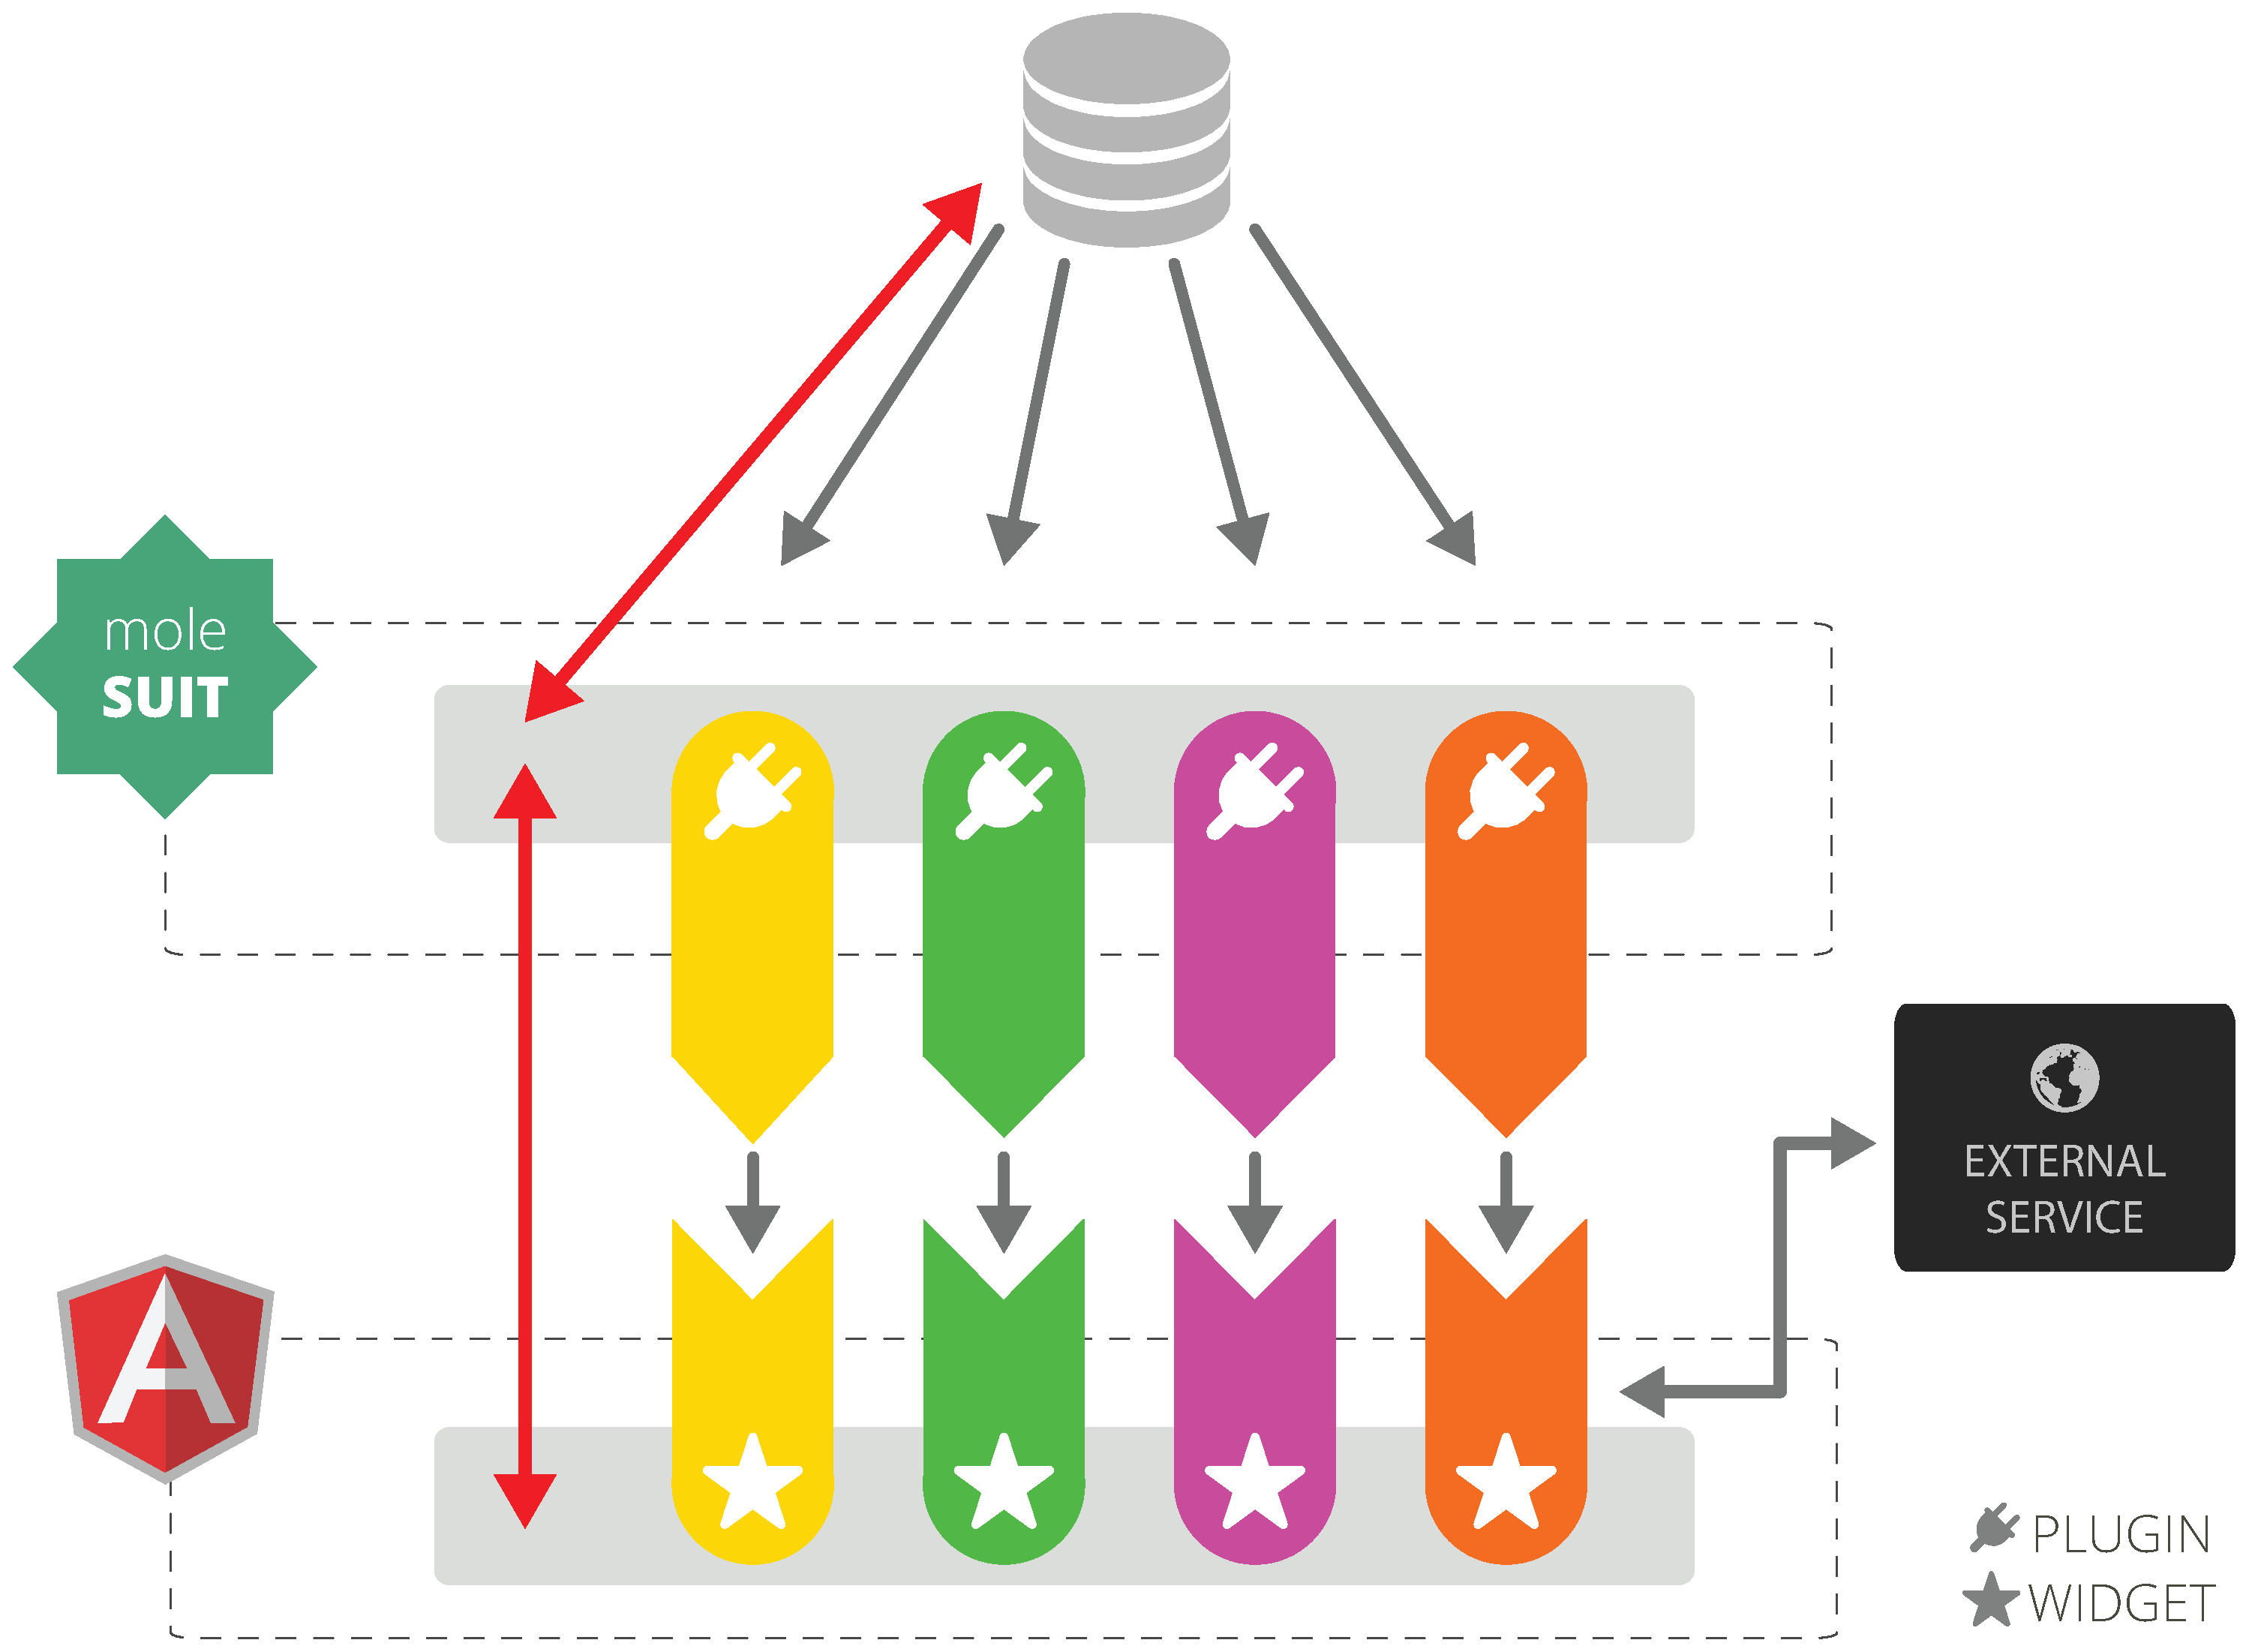
\includegraphics[width=1.0\linewidth]{./img/mole-suit}
\caption[Architettura di mole-suit]{Architettura di mole-suit}
\label{fig:mole-suit}
\end{figure}